%!TEX root = ../thesis.tex
% ******************************* Thesis Appendix A ****************************
\chapter{Schematics of the iPG instrument} 


\ifpdf
\graphicspath{{Appendix1/Figs/Raster/}{Appendix1/Figs/PDF/}{Appendix1/Figs/}}
\else
\graphicspath{{Appendix1/Figs/Vector/}{Appendix1/Figs/}}
\fi

\section*{Power supply}
\label{Appendix: Power Supply}
\begin{figure}[!htpb]
	\centering
	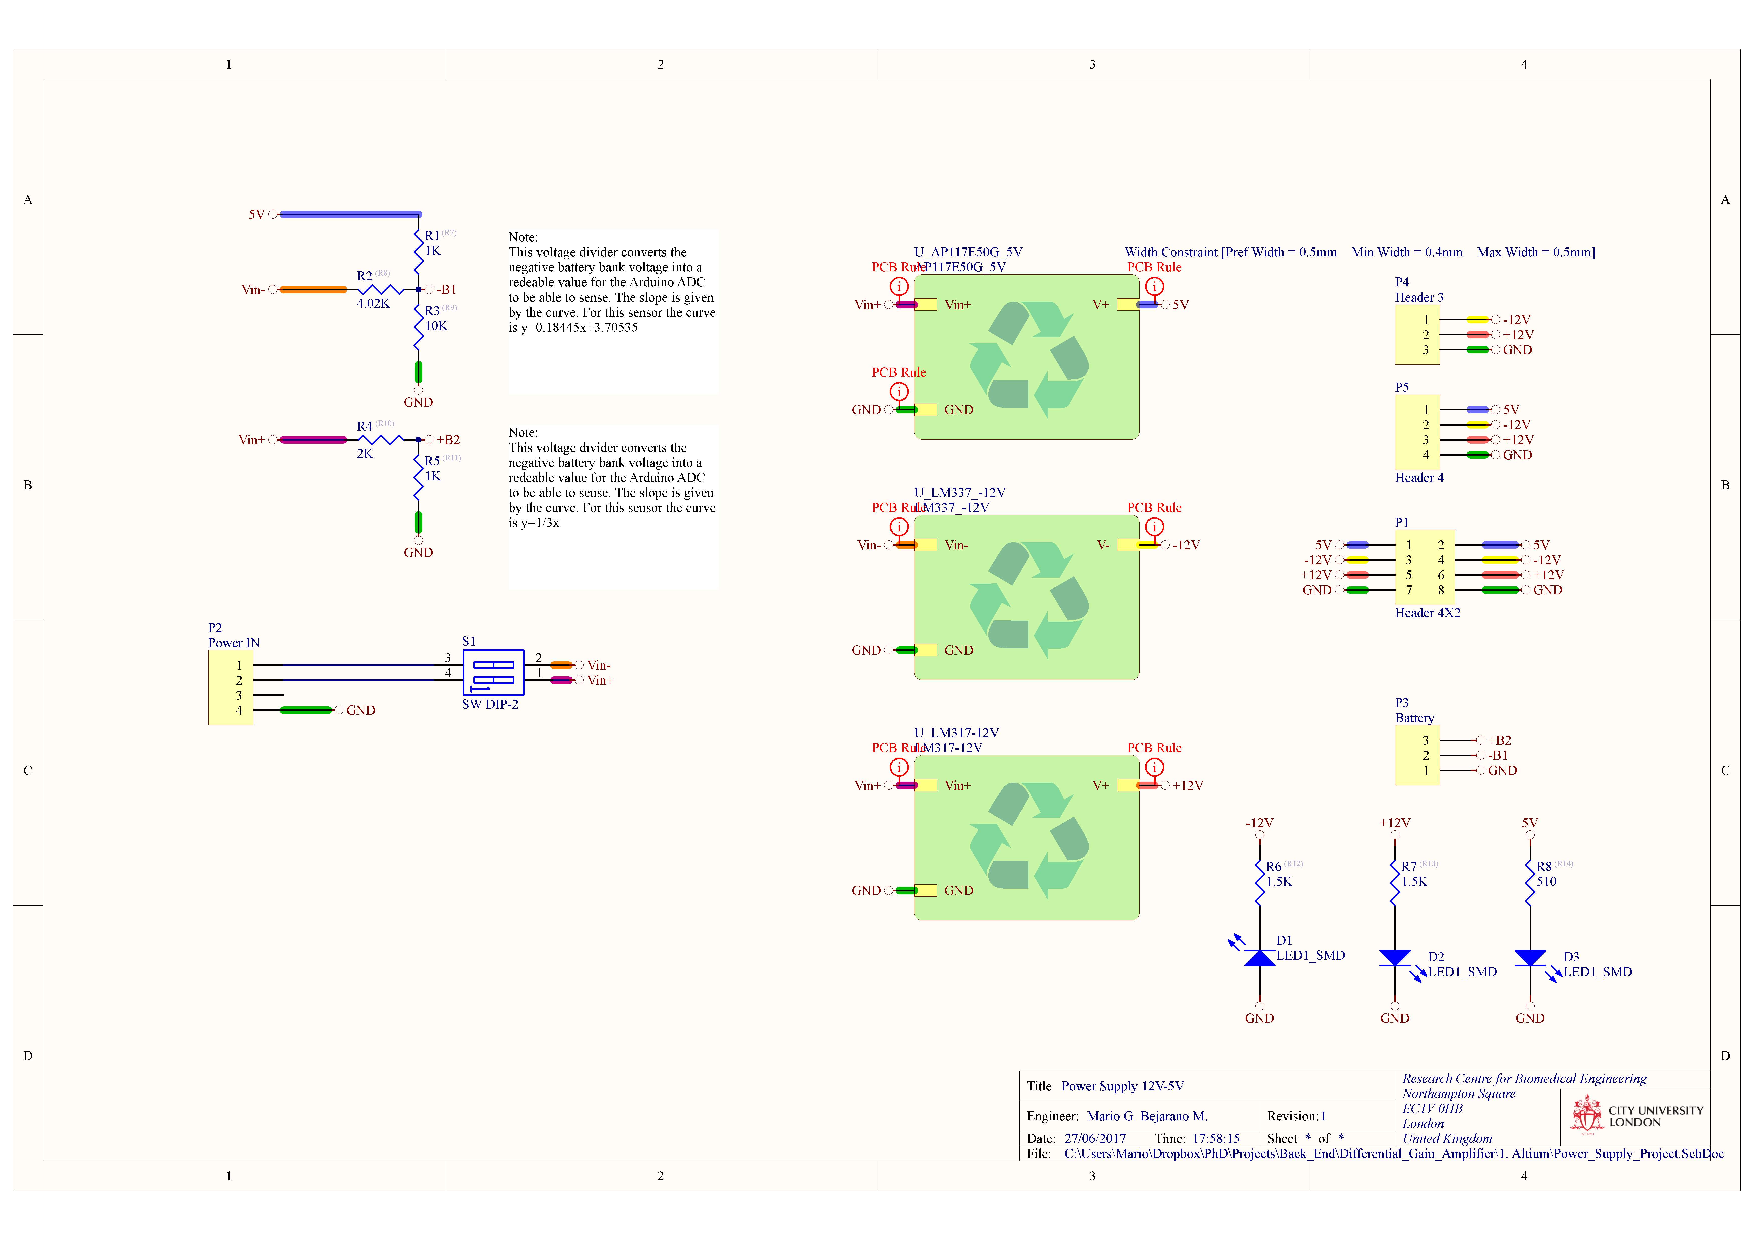
\includegraphics[width=0.55\paperwidth,keepaspectratio, angle=90]{power_supply_top}
	\caption[Top-up view of the power supply]{Top-up view of the power supply. Each box represents the Voltage regulators circuits. The schematic also includes indicators LED, switches and output ports.}
	\label{fig:schematic PS}
\end{figure}

\begin{landscape}
\begin{figure}[!htpb]
	\centering
	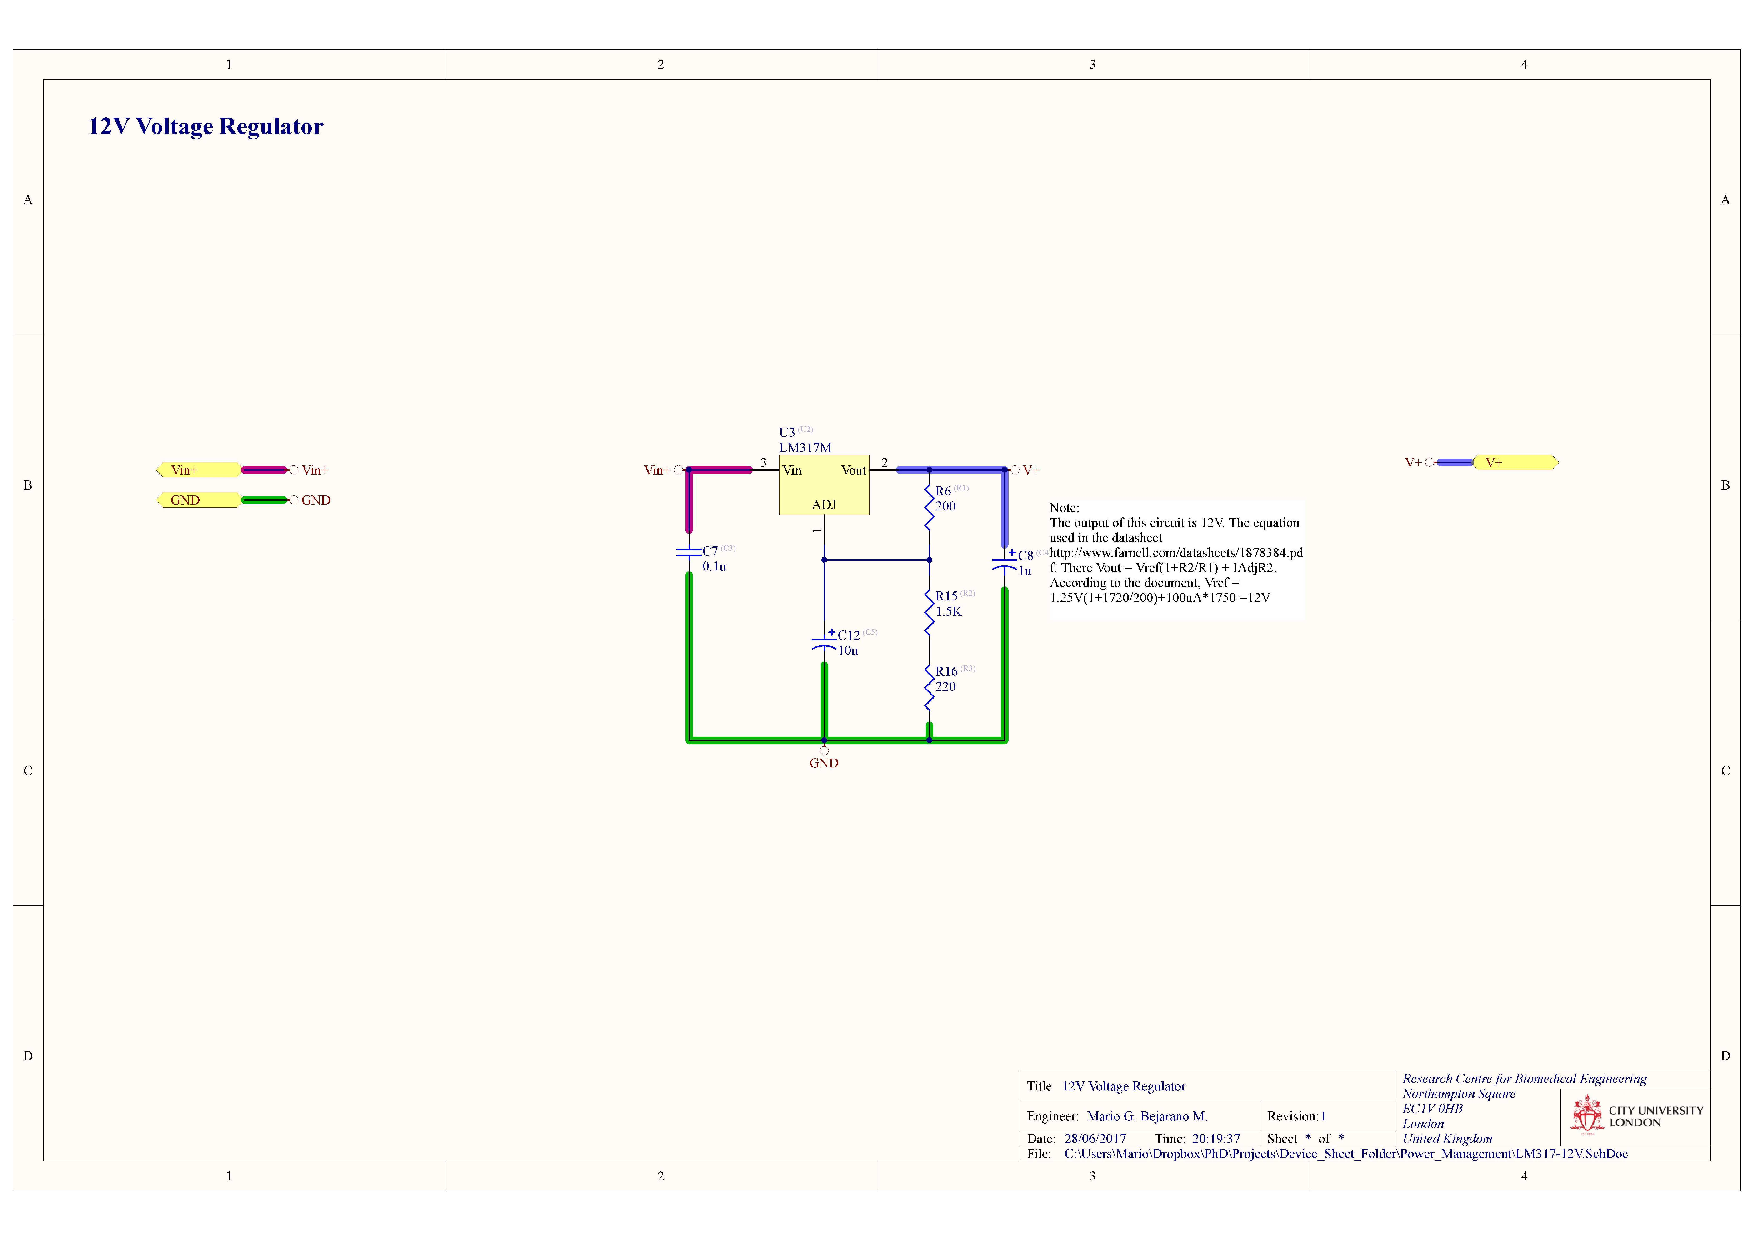
\includegraphics[width=\paperwidth,keepaspectratio]{power_supply_12}
	\caption[Schematic of the \SI{12}{\volt} voltage regulator]{The schematic shows the configuration of the voltage regulator LM317, the resistors selected set the output voltage at \SI{12}{\volt}. The capacitors filter ripples from the batteries.}
	\label{fig:schematic PS 12}
\end{figure}
\end{landscape}

\begin{landscape}
\begin{figure}[!htpb]
	\centering
	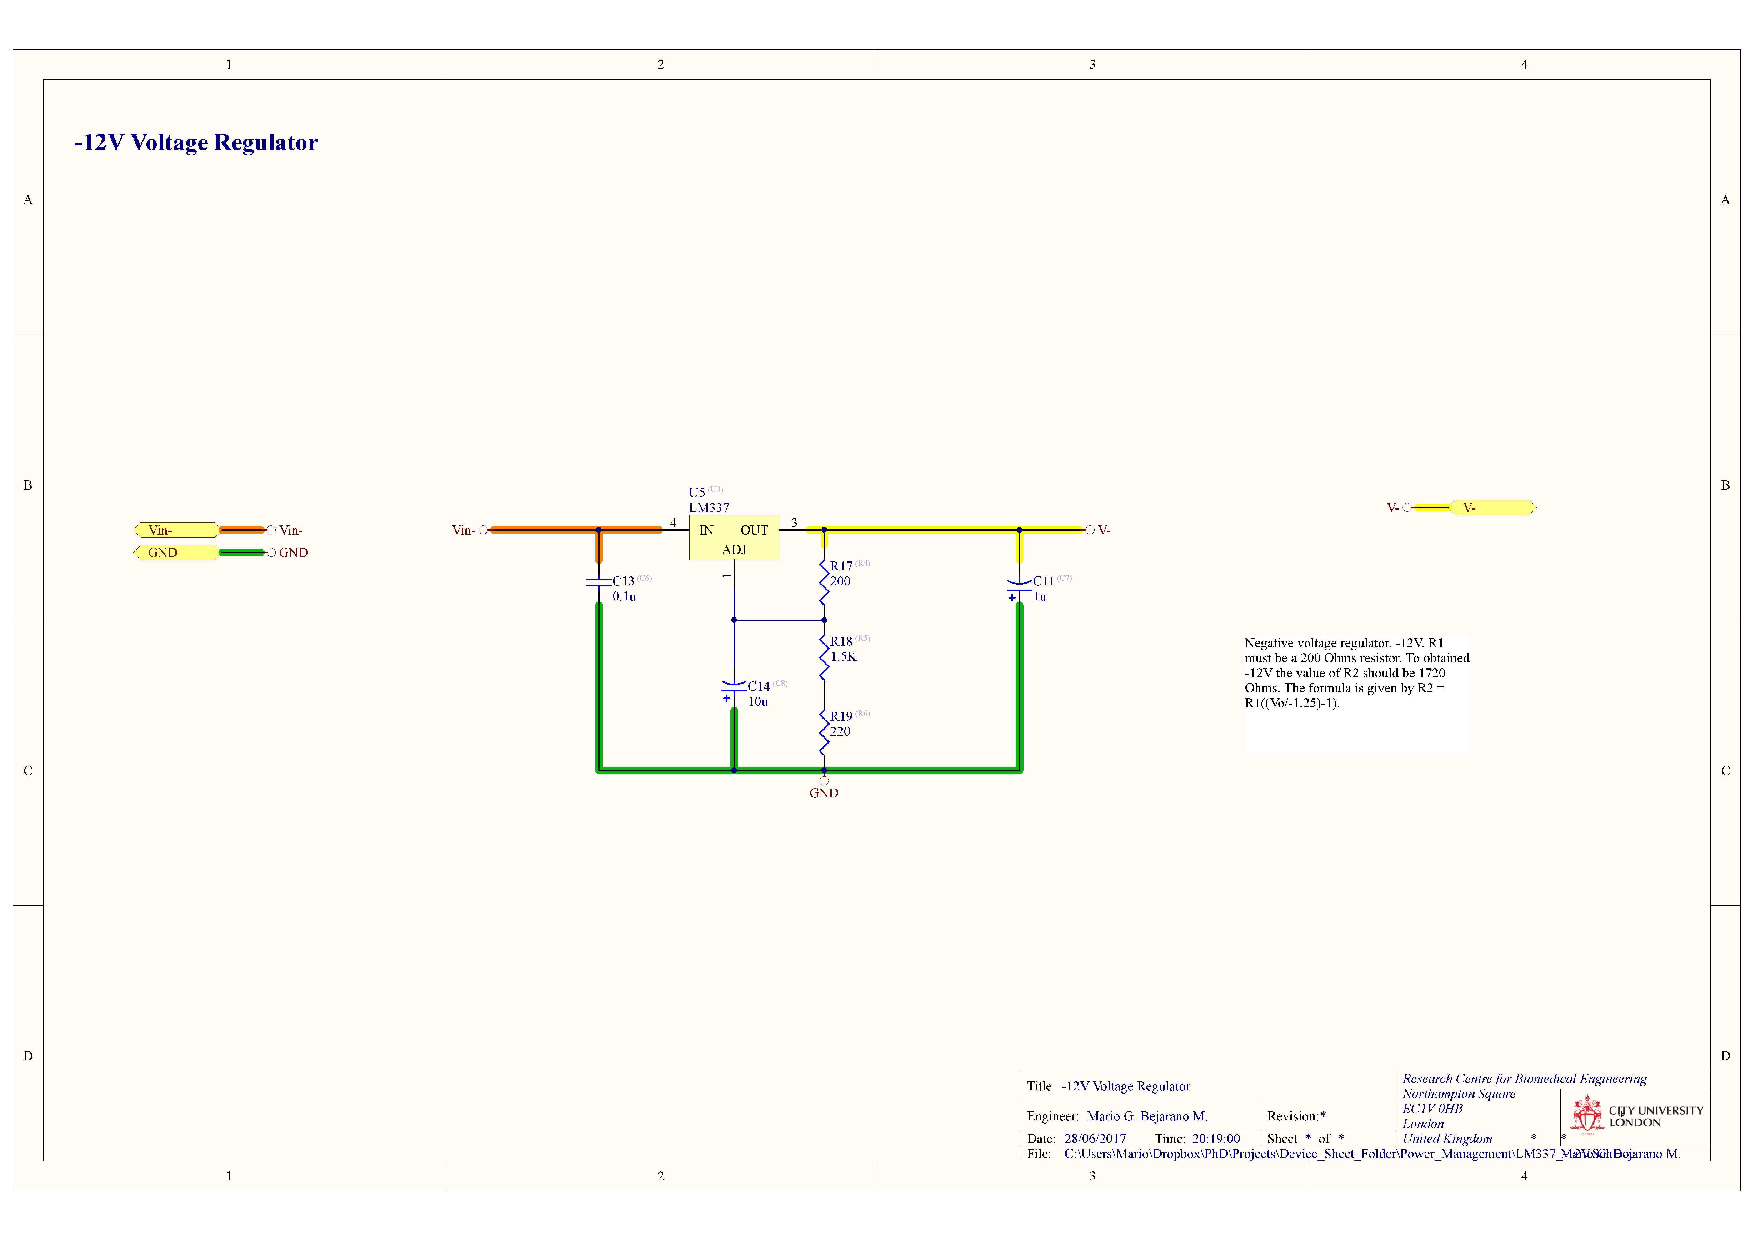
\includegraphics[width=\paperwidth,keepaspectratio]{power_supply_N12}
	\caption[Schematic of the -\SI{12}{\volt} voltage regulator]{The schematic shows the configuration of the voltage regulator LM337, the resistors selected set the output voltage at -\SI{12}{\volt}. The capacitors filter noise peaks.}
	\label{fig:schematic PS N12}
\end{figure}
\end{landscape}

\begin{landscape}
\begin{figure}[!htpb]
	\centering
	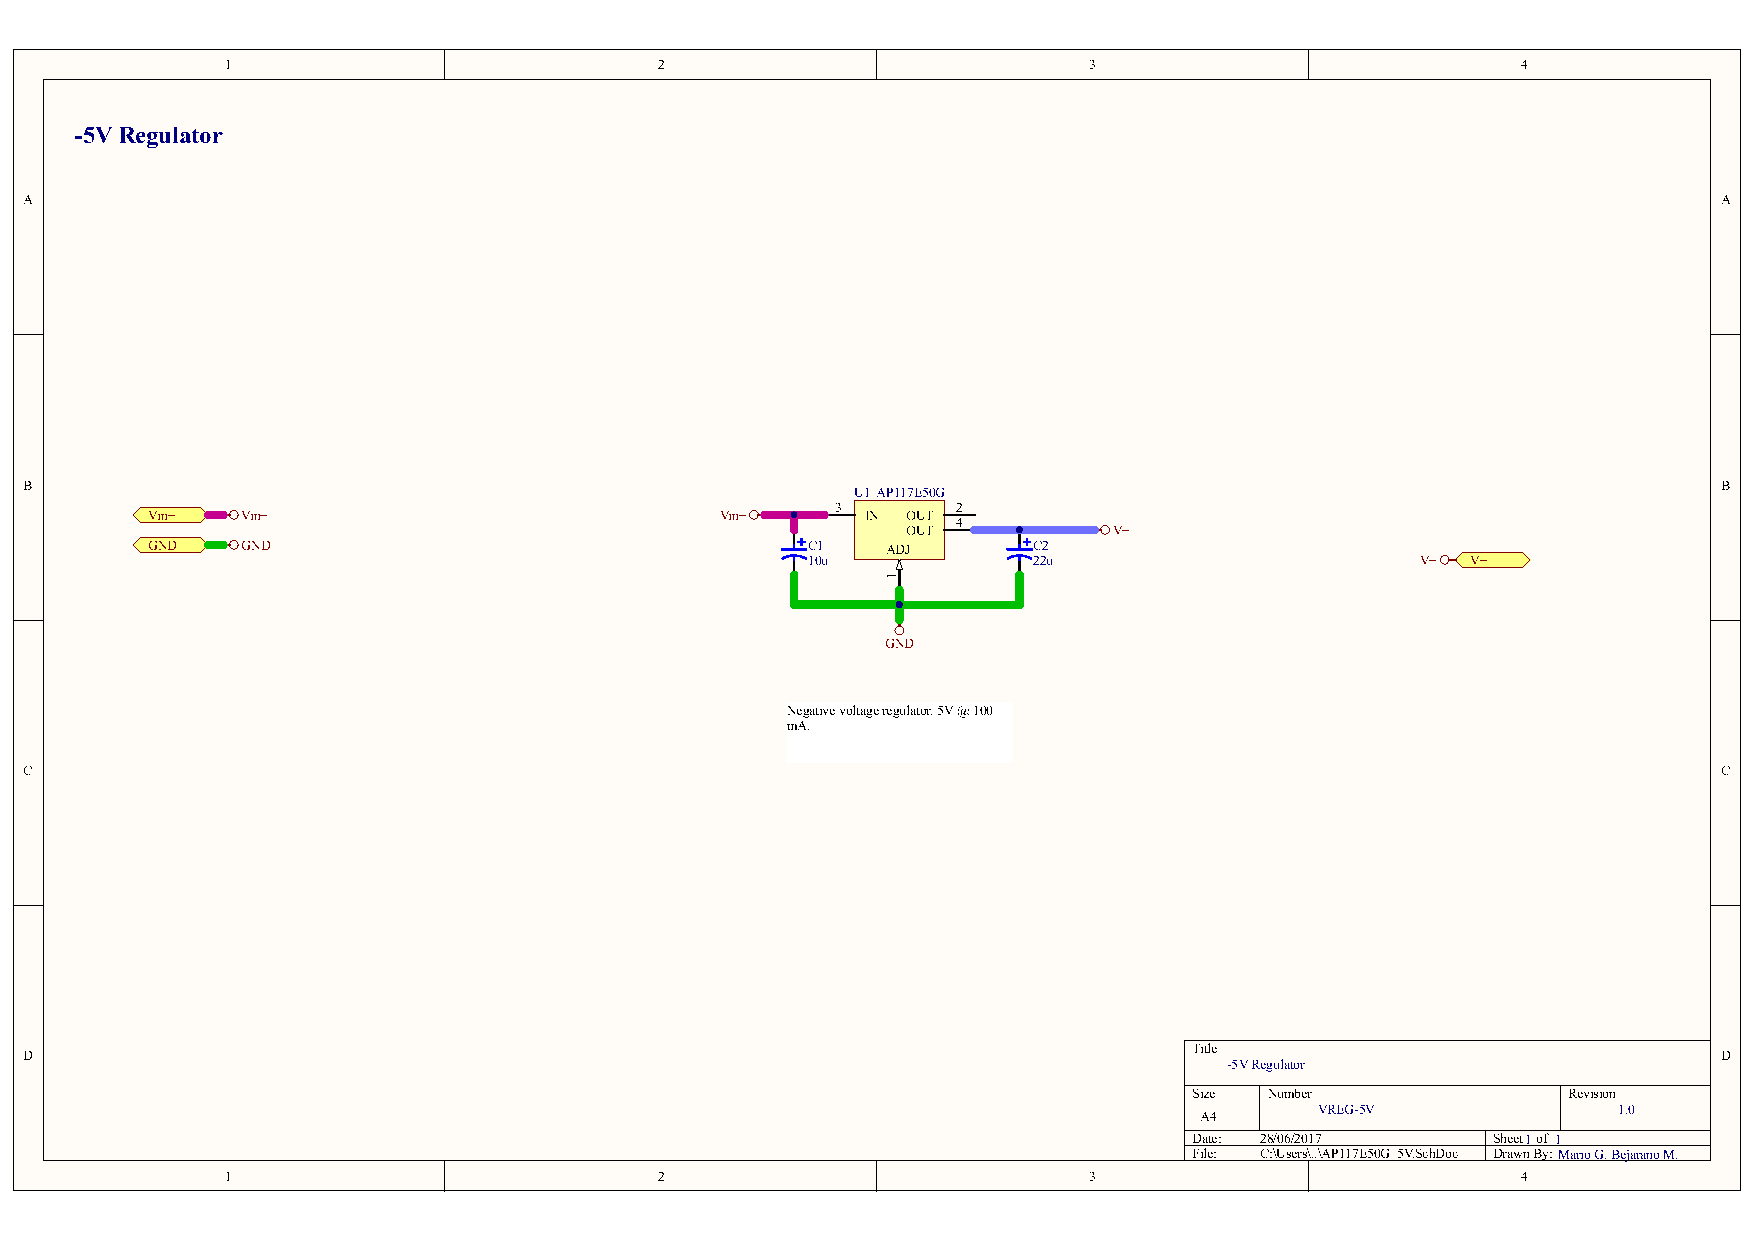
\includegraphics[width=\paperwidth,keepaspectratio]{power_supply_5}
	\caption[Schematic of the \SI{5}{\volt} voltage regulator]{The schematic shows the configuration of the voltage regulator AL117E50G, the output is fixed to \SI{5}{\volt}. The capacitors filter noises from the power bank.}
	\label{fig:schematic PS 5}
\end{figure}
\end{landscape}


\section*{DDS}
\label{Appendix: DDS PS}
\begin{figure}[!htpb]
	\centering
	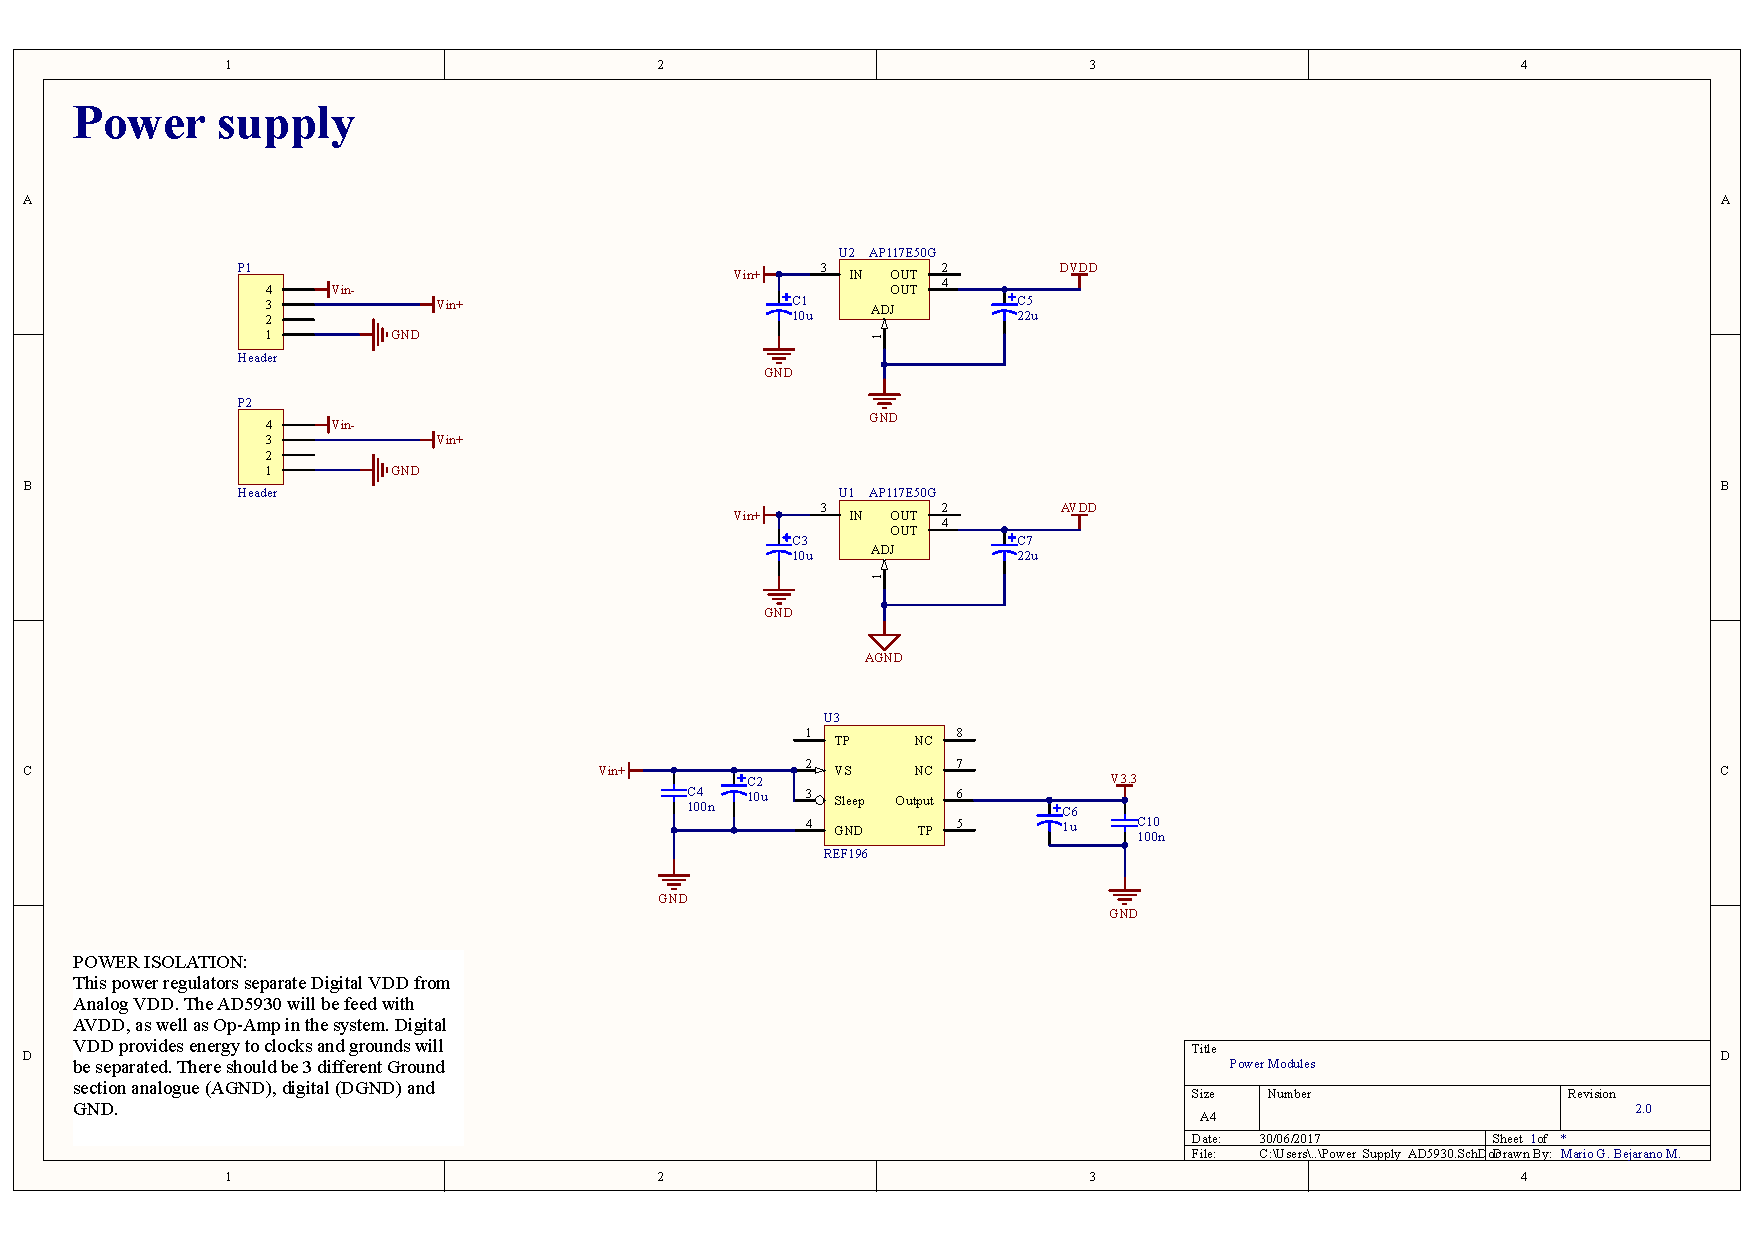
\includegraphics[width=0.9\paperwidth,keepaspectratio,angle=90]{DDS_power_supply}
	\caption[Schematic of the Power supply of the DDS]{The power supply circuit provides 3 different voltages \SI{5}{\volt} for analogue and digital circuitry, and \SI{3}{\volt} for voltage reference. There are three different ground paths for each source. }
	\label{fig:DDS PS}
\end{figure}


\begin{landscape}
	\begin{figure}[!htpb]
		\centering
		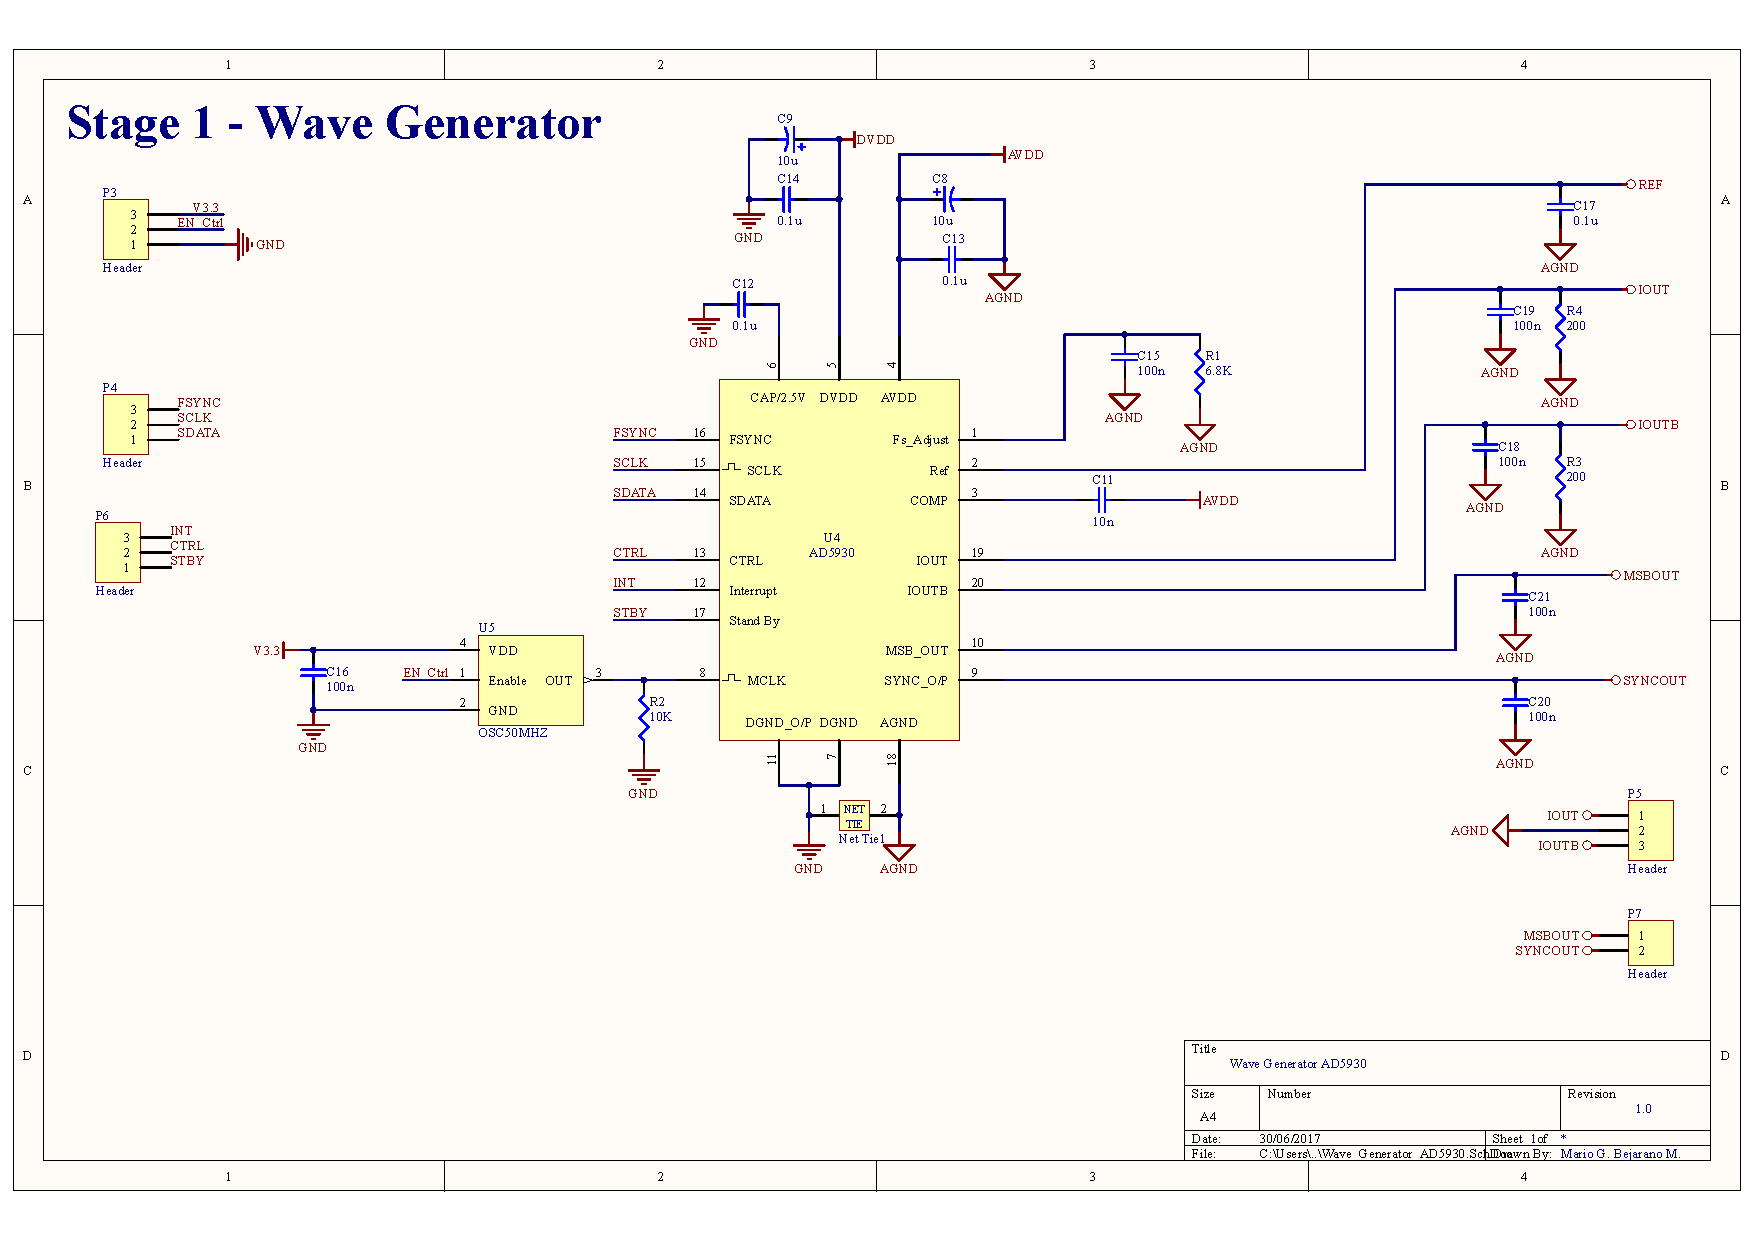
\includegraphics[width=\paperwidth,keepaspectratio]{DDS}
		\caption[Direct digital synthesis circuit schematic]{Schematic of the AD5930, it includes the \SI{50}{\mega\hertz} oscillator and output filters.}
		\label{fig:DDS}
	\end{figure}
\end{landscape}

\section*{Differential gain amplifier}
\label{Appendix: DGA}
\begin{figure}[!htpb]
	\centering
	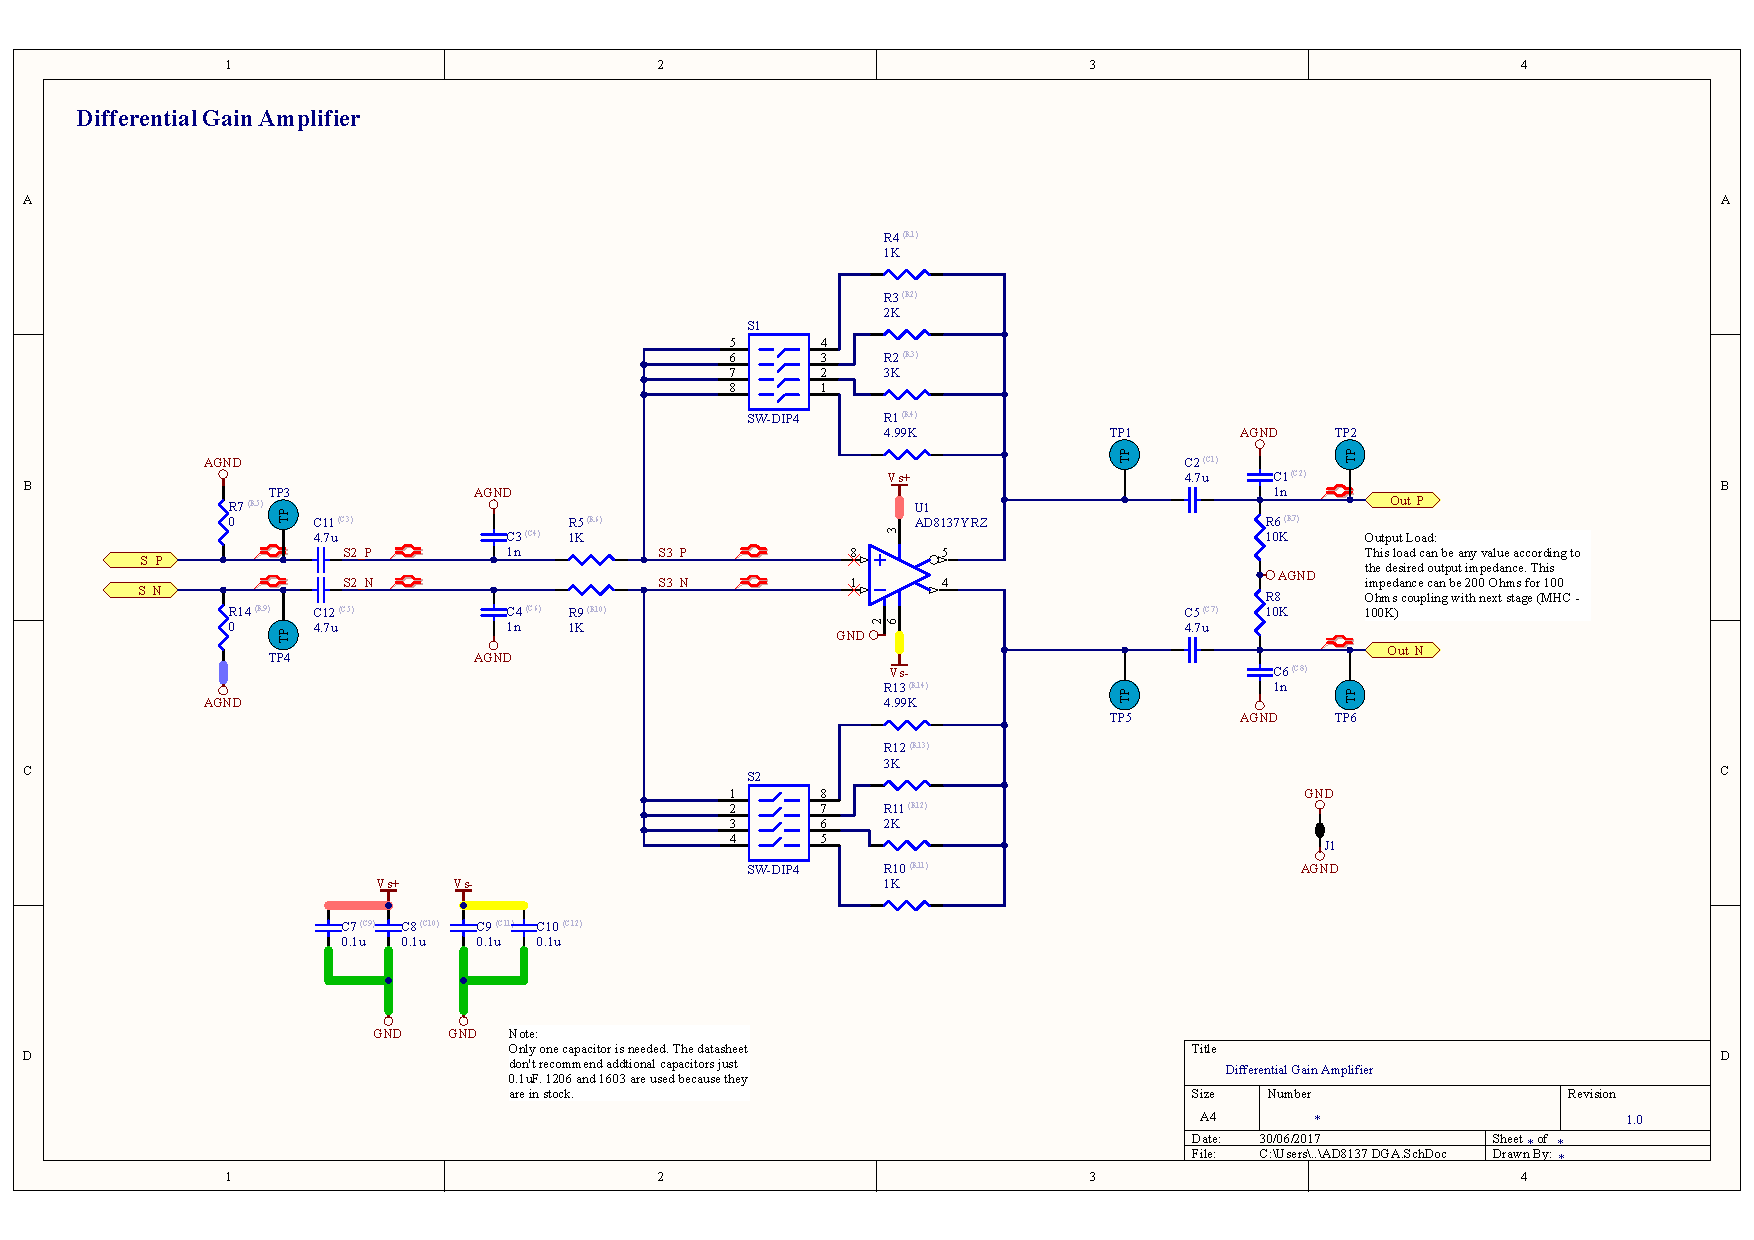
\includegraphics[width=0.9\paperwidth,keepaspectratio,angle=90]{DGA}
	\caption[Schematic of the differential gain amplifier circuit]{Differential gain amplifier controlled by 4 position dip-switch adjusting the gain of the signal output.}
	\label{fig:DGA}
\end{figure}

\begin{landscape}
	\begin{figure}[!htpb]
		\centering
		\includegraphics[width=\paperwidth,keepaspectratio]{DDS_PS_6}
		\caption[Positive power supply (\SI{6}{\volt}) for the differential amplifier]{Power supply circuit based on the IC LF60CDT.}
		\label{fig:DGA PS 6}
	\end{figure}
\end{landscape}

\begin{landscape}
	\begin{figure}[!htpb]
		\centering
		\includegraphics[width=\paperwidth,keepaspectratio]{DDS_PS_N6}
		\caption[Negative power supply (\SI{-6}{\volt}) for the differential amplifier]{Power supply circuit based on the IC LM337, the resistors were adjusted to achieve -\SI{6}{\volt}.}
		\label{fig:DGA PS -6}
	\end{figure}
\end{landscape}

\section*{Modified Howland circuit}

\section*{Voltage sense circuit}